\documentclass{article}
\usepackage[utf8]{inputenc}
\usepackage[document]{ragged2e}
\usepackage{algpseudocode}
\usepackage[]{algorithmicx}
\usepackage{amsmath}
\usepackage{amsthm}
\usepackage{amssymb}
\usepackage[]{listings}
\usepackage{graphicx}
\usepackage{hyperref}
\usepackage{flafter}
\usepackage{subfig}
\usepackage{dsfont}
\graphicspath{ {images/} }

\begin{document}

\begin{titlepage}
	\centering
	
\includegraphics[width=0.15\textwidth]{IIIT-B_logo.jpg}\par\vspace{1cm}
	{\scshape\LARGE International Institute of Information Technology, Bangalore \par}
	\vspace{1cm}
	{\scshape\Large Milestone IV \par}
	{\Large  DS 707 Data Analytics\par}
	\vspace{1.5cm}
	{\huge\bfseries Clustering and Association Rules Mining \par}
	\vspace{2cm}
	{\Large\itshape Akanksha Dwivedi - MT2016006\par}
	{\Large\itshape Hitesha Mukherjee - MS2016007\par}
	{\Large\itshape Nayna Jain - MS2017003\par}
	{\Large\itshape Tarini Chandrashekhar - MT2016144\par}
	\vfill
	Instructors : \par
	Prof. Ramanathan Chandrashekhar
	\par
	Prof. Uttam Kumar

	\vfill
% Bottom of the page
	{\large \today\par}
\end{titlepage}

\newpage

\tableofcontents

\newpage
\justify


\section{Introduction to Clustering}
Clustering is the task of dividing the population or data points into a number of groups such that data points in the same groups are more similar to other data points in the same group than those in other groups. \newline

There are many clustering methods available, and each of them may give a different grouping of a Dataset. The choice of a particular method will depend on the type of output desired, The known performance of method with particular types of data, the hardware and software facilities available and the size of the Dataset. 

\section{Chameleon: A Hierarchical Clustering Algorithm}

Hierarchical clustering algorithm called CHAMELEON that measures the similarity of two clusters based on a dynamic model. In the clustering process, two clusters are merged only if the inter-connectivity and closeness (proximity) between two clusters are comparable to the internal inter-connectivity
of the clusters and closeness of items within the clusters.

\subsection{Inferences Drawn from our Dataset}
We have considered the Bitcoin Data Set which has 24 features or attributes in it. We have extracted 16 important features and build a subset of the data. This Dataset has been clustered using Chameleon. From Figure 1 we see that we have six clusters of different size, shape, and orientation, as well as random noise points and special artifacts such as streaks running across clusters.In this case CHAMELEON finds eleven clusters, out of which six of them correspond to the genuine clusters in the data set, and the rest contain outliers.\newline


\begin{figure}[h]
    \centering
    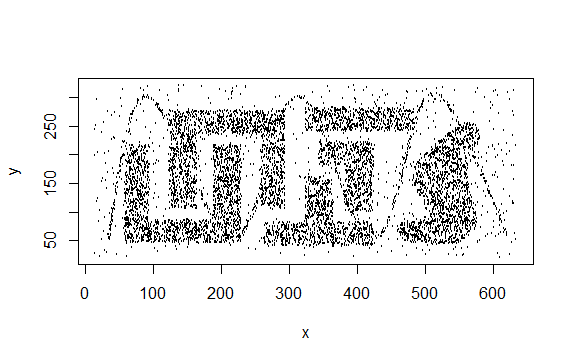
\includegraphics[width=10cm]{chameleonBitcoinFig1.png}
    \caption{Chameleon Clustering Bitcoin}
    \label{fig:my_label}
\end{figure}


The next data set is etherium Dataset with 12 attributes. From Figure 2 we see it has eight clusters of different shape, size, and orientation, some of which are inside the space enclosed by other clusters. Moreover, it also contains random noise and special artifacts, such as a collection of points forming vertical streaks. In this case CHAMELEON also finds eleven clusters, out of
which nine of them correspond to the genuine clusters, and the rest contain outlier points.\newline

\begin{figure}[h]
    \centering
    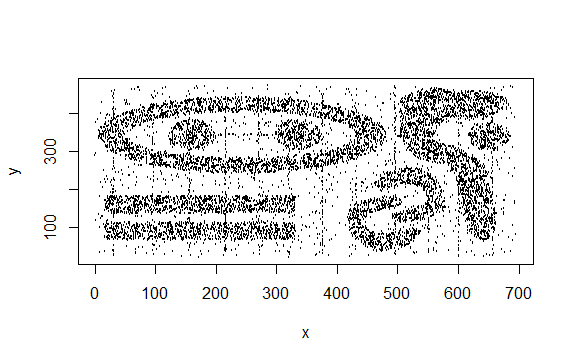
\includegraphics[width=10cm]{ChameleonEtheriumFig2.png}
    \caption{Chameleon Clustering Etherium}
    \label{fig:my_label}
\end{figure}

Since CHAMELEON is hierarchical in nature, it creates a Dendrogram of possible clustering solutions at different levels of granularity. The clustering solutions shown in these Figures correspond to the earliest point in the Agglomerative process in which CHAMELEON was able to find the genuine clusters in the data set. That is, they correspond to the lowest level of the Dendrogram at which the genuine clusters in the data set have been identified and each one has been
placed together in one cluster. As a result, the number of clusters shown in these figures for each one of the data sets can be larger than the number of genuine clusters, and these additional clusters contain points that are outlier.

\section{CLARANS - Partitioning around Mediods}

CLARANS (Clustering Large Applications based upon
RANdomized Search ) was proposed to improve the quality and the scalability of CLARA. It combines sampling techniques with PAM.It does not confine itself to any sample at a given time.
It draws a sample with some randomness in each step of the search. \newline

Advantages
\begin {itemize}
\item Experiments show that CLARANS is more effective than both PAM
and CLARA
\item Handles outliers 

Disadvantages
\item The computational complexity of CLARANS is O(n2), where n is the
number of objects
\item The clustering quality depends on the sampling method
\end{itemize}


\subsection{Inferences Drawn from our Dataset}
We take the Bitcoin Dataset into consideration. It has 16 attributes. We have considered 2 attributes(Market Price Label and Market Cap)  for CLARANS Clutering. From Figure 3, we observe that the Market Cap and Market Price varies almost in the same way for negative and positive values. It means that they are highly correlated. There is a similarity in their pattern, hence the clusters are based on similarity measure. We  have used Euclidean Distance Parameter for Computation. \newine

\begin{figure}[h]
    \centering
    \includegraphics[width=10cm]{CLaransClustering.png}
    \caption{Clarans Clustering for Market Price and Market Cap }
    \label{fig:my_label}
\end{figure}



\begin{figure}[h]
    \centering
    \includegraphics[width=10cm]{CLARANSMARCAPVOL.png}
    \caption{Clarans Clustering for Market Cap and Volume }
    \label{fig:my_label}
\end{figure}

The next dataset BitCoin Price Dataset we considered has 7 attributes. From Figure 4, we have considered 2 attributes(Volume and Market Cap) for CLARANS Clutering. We observe a certain randomness about the clusters. No similarity pattern is observed. The volume and Market Cap vary randomly.

\section{DBSCAN - Density-Based Clustering}
Density-based clustering is a technique that allows to partition data into groups with similar characteristics (clusters) but does not require specifying the number of those groups in advance. In density-based clustering, clusters are defined as dense regions of data points separated by low-density regions. Density is measured by the number of data points within some radius.\newline

Advantages of density-based clustering:
As mentioned above, it does not require a predefined number of clusters,clusters can be of any shape, including non-spherical ones,the technique is able to identify noise data (outliers).\newline

Disadvantages:\newline
Density-based clustering fails if there are no density drops between clusters, it is also sensitive to parameters that define density (radius and the minimum number of points); proper parameter setting may require domain knowledge.

\subsection{Inferences Drawn from our Dataset}
This algorithm works on a parametric approach. The two parameters involved in this algorithm are:
e - (eps) is the radius of our neighborhoods around a data point p.
minPts (K)- It is the minimum number of data points we want in a neighborhood to define a cluster.Using these two parameters, DBSCAN categories the data points into three categories:
Core Points: A data point p is a core point if Nbhd(p,eps) [eps-neighborhood of p] contains at least minPts; \mathopen|Nbhd(p,eps)|$\geq$ minPts.
Border Points: A data point *q is a border point if Nbhd(q, eps) contains less than minPts data points, but q is reachable from some core point p.
Outlier: A data point o is an outlier if it is neither a core point nor a border point. Essentially, this is the "other" class. \newline

The idea is to calculate, the average of the distances of every point to its k nearest neighbors. The value of k will be specified by the user and corresponds to MinPts.We have used K-Nearest Neighbour Algorithm to determine the K value (minPts) to be used as a parameter for the DBSCAN Algorithm. The minimum value obtained for K was 5. \newline

The value of epsilon is calculated in the following manner. The function kNNdistplot() [in dbscan package] can be used to draw the k-distance plot. k-distances are plotted in an ascending order. The aim is to determine the “knee”, which corresponds to the optimal eps parameter. \newline

A knee corresponds to a threshold where a sharp change occurs along the k-distance curve. From Figure 5, It can be seen that the optimal eps value is around a distance of 0.15.


\begin{figure}[h]
    \centering
    \includegraphics[width=10cm]{epswith2attr.png}
    \caption{K-Distance Curve for determining Eps Value }
    \label{fig:my_label}
\end{figure}

We take the Bitcoin Dataset into consideration. It has 16 attributes. We have considered 2 attributes(Total Bitcoins and Market Cap) for DBSCAN Clustering.\newline

From Figure 6, the variation of Total Bitcoins and Market Cap is constant for negative values, but as the value increases, we observe a sharp spike after zero for total BitCoins with respect to the Market Cap. The blue Cluster has maximum density, it is densely connected and has maximum density reachable value. We observe there are two outliers in the dataset. \newline

\begin{figure}[h]
    \centering
    \includegraphics[width=10cm]{PlotMarCapTotCoins.png}
    \caption{DBSCAN Clustering for Total Coins and Market Cap }
    \label{fig:my_label}
\end{figure}


\begin{figure}[h]
    \centering
    \includegraphics[width=10cm]{totbitcoinstradevol.png}
    \caption{DBSCAN Clustering for Total Coins and Trade Volume }
    \label{fig:my_label}
\end{figure}

We have considered 2 attributes Total Bitcoins and Trade Volume for DBSCAN Clustering. From Figure 7, we observe that there is sharp change in the value of Total Bitcoins and Trade Volume. Also there is an overlap of clusters(Blue Cluster and Gray Cluster).The entire Blue Cluster and some parts of the Gray Cluster can be considered as core points and the remaining parts of gray cluster are the Border Points. There are 2 points away from the clusters one is yellow point and the other single gray point, which can be termed as outliers. \newline

\begin{figure}[h]
    \centering
    \includegraphics[width=10cm]{dbmarcapvol.png}
    \caption{DBSCAN Clustering for Market Cap and Trade Volume }
    \label{fig:my_label}
\end{figure}


We have considered 2 attributes Market Cap and Trade Volume for DBSCAN Clustering. From Figure 8, we observe that the first cluster is very dense. The second and third clusters are very sparse. We observe that as the Market Cap increases the clusters become less denser, After the market cap and trade volume crosses the value of 5 in the x and y axis we observe very few points lie on that region. We can therefore conclude that both Market Cap and Trade Volume are directly proportional to each other. We also observe 2 outliers in the dataset.

\section {Association Rules Mining}
Association rule learning is a rule-based machine learning method for discovering interesting relations between variables in large databases. It is intended to identify strong rules discovered in databases using some measures of interestingness It is often used by grocery stores, retailers, and anyone with a large transactional databases.Association rules use the R arules library. The arulesViz add additional features for graphing and plotting the rules. 

\subsection{Inferences Drawn from our Dataset}
We have considered the Bitcoin Data Set which has 24 features or attributes in it. We have extracted 16 important features and build a subset of the data.First we have converted our dataset to transactions which is necessary step for rule creation. The rules can then be created using the Apriori function on the transaction dataset. After running the Apriori Function 860931 rules were created and the following statistics were obtained; Confidence of 0.8 and Minimum Support count of 292. The figure 9 illustrates it. \newline


\begin{figure}[h]
    \centering
    \includegraphics[width=10cm]{RuleMiningScatterPlot.png}
    \caption{ Association Rule Mining Scatter Plot }
    \label{fig:my_label}
\end{figure}


After sorting the top three rules based on "Lift",we have inferred the following that 2 attributes Transaction to Trade Ratio and  Estimated Transaction Volume have highest Support, Confidence and Lift Count Statistics. If the rule had a lift of 1, it would imply that the probability of occurrence of the antecedent and that of the consequent are independent of each other. When two events are independent of each other, no rule can be drawn involving those two events.\newline

If the lift is $>$ 1, that lets us know the degree to which those two occurrences are dependent on one another, and makes those rules potentially useful for predicting the consequent in future data sets. \newline

The value of lift is that it considers both the confidence of the rule and the overall data set.The next attribute Market Price Label has slight lesser value of Support, Confidence and Lift Count than the above mentioned attributes. We have used arulesViz package for visualization and obtained the Two-Key Plot IN Figure 10 which maps support on x-axis and confidence on y-axis from highest order to lowest order. 

\begin{figure}[h]
    \centering
    \includegraphics[width=10cm]{rules2plot.png}
    \caption{ Two Key Plot for Mapping Support and Confidence}
    \label{fig:my_label}
\end{figure}

 We can now the subset of rules to get a visual on the rules. Every rule is composed by two different sets of items, also known as itemsets,  X and Y, where X is called antecedent or left-hand-side (LHS) and Y consequent or right-hand-side (RHS).From figure 11 we get these graphs we can see the two parts to an association rule: the antecedent (IF) and the consequent (THEN).  These patterns are found by determining frequent patterns in the data and these are identified by the support and confidence.  The support indicates how frequently the items appear in the dataset. The confidence indicates the number of times the IF/THEN statement on the data are true. These IF/THEN statements can be visualized by the following graph. \newline
 
 \begin{figure}[h]
    \centering
    \includegraphics[width=10cm]{AntecedentConsequent.png}
    \caption{AntecedentConsequent for the Subrules Created}
    \label{fig:my_label}
\end{figure}

 \begin{figure}[h]
    \centering
    \includegraphics[width=10cm]{Graphfor30Rules.png}
    \caption{Graph for 30 Rules}
    \label{fig:my_label}
\end{figure}

We can then subset the rules to the top 30 most important rules and then inspect the smaller set of rules individually to determine where there are meaningful associations. We plot the graph (Figure 12) for top 30 rules and inspect them to find meaningful correlation between different attributes based on LHS and RHS. In practical applications, a rule needs a support of several hundred transactions before it can be considered statistically significant and datasets often contain thousands or millions of transactions.

\end{document}
